\documentclass[a4paper,11pt]{kth-mag}
\usepackage[T1]{fontenc}
\usepackage{textcomp}
\usepackage{lmodern}
\usepackage[utf8]{inputenc}
\usepackage[swedish,english]{babel}
\usepackage{modifications}
\usepackage{graphicx}
\usepackage{blindtext}
\usepackage{tabularx}
\usepackage{listings}

% No images or other floats can pass through \FloatBarrier 
\usepackage{placeins}

\title{A study of Sudoku solving algorithms}
\subtitle{}
\foreigntitle{En studie om Sudokulösningsalgorithmer}
\author{Patrik Berggren \and David Nilsson}
\date{April 2012}
\blurb{Bachelor's Thesis at NADA\\Supervisor: Alexander Baltatzis\\Examiner: Mårten Björkman}
\trita{TRITA xxx yyyy-nn}
\begin{document}
\frontmatter
\pagestyle{empty}
\removepagenumbers
\maketitle
\selectlanguage{english}
\begin{abstract}
In this bachelor thesis three different Sudoku solving algorithms are studied.
The study is primarly concerned with solving ability, but also includes the following: difficulty rating, puzzle generation ability, and suitability for parallelizing.
These aspects are studied for individual algorithms but are also compared between the different algorithms.
The evaluated algorithms are backtrack, rule-based and Boltzmann machines.
Measurements are carried out by measuring the solving time on a database of 17-clue puzzles, with easier versions used for the Boltzmann machine.
Results are presented as solving time distributions for every algorithm, but relations between the algorithms are also shown.
We conclude that the rule-based algorithm is by far the most efficient algorithm when it comes to solving Sudoku puzzles.
It is also shown that some correlation in difficulty rating exists between the backtrack and rule-based algorithms.
Parallelization is applicable to all algorithms to a varying extent, with clear implementations for search-based solutions.
Generation is shown to be suitable to implement using deterministic algorithms such as backtrack and rule-based.

\end{abstract}
\clearpage
\begin{foreignabstract}{swedish}
Den här exjobbsrapporten på kandidatnivå presenterar tre olika lösningsalgoritmer för Sudoku.
Studiens huvudsyfte är att studera lösningsprestanda men analyserar även svårighetsgrad, möjligheter till generering och parallelisering.
Samtliga aspekter studeras för varje algoritm och jämförs även mellan enskilda algoritmer.
De utvalda algoritmerna är backtrack, regelbaserad och Boltzmann-maskiner.
Samtliga mätningar görs på en databas med pussel som har 17 ledtrådar, med vissa anpassningar för Boltzmann-maskiner.
Resultaten presenteras med fördelningar som visar lösningstider för varje algoritm separat. 
Slutsatsen är att regelbaserade lösare är effektivast på att lösa Sudokupussel.
En korrelation mellan den regelbaserades och den backtrack-baserade lösares svårighetsrating visas.
Parallelisering visas vara tillämpbart till olika grad för de olika algoritmerna och är enklast att tillämpa på sökbaserade lösare.
Generering konstateras vara lättast att implementera med deterministiska algoritmer som backtrack och rule-based.
\end{foreignabstract}
\clearpage
\section{Statement of collaboration}
This is a list of responsibilities:
\begin{itemize}
    \item Implementations: Patrik has been responsible for the rule-based solver and the backtrack solver. David has been responsible for the Boltzmann machine and the test framework.
    \item Analysis: Patrik has analyzed data from the rule-based solver and the backtrack solver. David has analyzed data from the Boltzmann machine.
    \item Report writing: Patrik has written the first draft of introduction and method. David has written the first draft of background and conclusions. The analysis part was written together. Reviewing of the whole report was also a divided responsibly.
\end{itemize}

\clearpage
\tableofcontents*
\clearpage
\listoffigures*
\mainmatter
\pagestyle{newchap}

\chapter{Introduction}
Sudoku is a game that under recent years have gained popularity.
Many newspaper today contain Sudoku puzzles and there are even competitions devoted to Sudoku solving.
It is therefore of interest to study how one can solve, generate and rate such puzzles by the help of computer algorithms. This thesis explores these concepts for a three chosen algorithms.

\FloatBarrier
\section{Problem specification}
There exists multiple algorithms for solving Sudoku puzzles.
This report is limited to the study of three different algorithms, each representing different solving approaches.
Primarly the focus is to measure and analyse those after solving ability.
There is however also other aspects that will be covered in this thesis.
Those are difficulty rating, Sudoku puzzle generaton, and how well the algorithms is suited for parallelizing.
The goal of this thesis is therefore to conclude how well each algorithm performs at these aspects, but also how they compare relative to one another.
Another goal is to see if any conclusions regarding Sudoku puzzles in general can be drawn.
The chosen algorithms for evaluation are backtrack, rule-based and Boltzmann machines.
All algorithms with their respective implementation issues are further discussed in section~\ref{sec:background} (background).

\FloatBarrier
\section{Scope}
As this project is quite limited in time and in expected scope, 
there are several limitations. The most noteable of those limitations are listed below: 
\begin{itemize}
    \item Limited number of algorithms:
There are as mentioned several other Sudoku solving algorithms. The chosen algorithms can also be modified and studied to determine which variation gives what properties. We have as mentioned limited the number of algorithms to three and we are also very restrictive in which variations we study.  
    \item Optimization: 
All algorithms are implemented by ourselfes and optimization is therefore an issue. 
We have therefore only aimed for exploring the underlying ideas of the algorithms and not the algorithms themselfes.
This means that some implementations may consciously be made in a certain way even if known optimizations are known.

    \item Special Sudokus: There are several variations of Sudoku including different sizes of the grid.
This thesis is, however, limited to the study of ordinary Sudoku, which is 9x9 grids.
\end{itemize}

\FloatBarrier
\section{Purpose}
As already mentioned, Sudoku is today a popular game throughout the world and it appears in multiple medias, including websites, newspapers and books. 
As a result, it is of interest to find effective Sudoku solving and generating algorithms. 
For most purposes there already exist satisfactory algorithms, and one might therefore struggle to see the use in studying Sudoku solving algorithms. 
There is, however, still some value in studying Sudoku solving algorithms as it might reveal how one can deal with harder variations of Sudoku, such as puzzles with 16x16 grids. 
Sudoku is also, as will be discussed in section~\ref{sec:background}, an NP-Complete problem which means that it is one of a set of computational difficult problems.\cite{complexity} 
One hope of this study is therefore to contribute to the discussion about how one can deal with such puzzles. 

\subsection{Definitions}
\begin{description}
    \item[Box:] A 3x3 grid inside the Sudoku puzzle. It works the same as rows and columns, meaning it must contain the digits 1-9.
    \item[Region:] This refers to a row, column or box.
    \item[Candidate:] An empty square in a Sudoku puzzle have a certain set of numbers that does not conflict with the row, column and box it is in. Those numbers are called candidates or candidate numbers.
    \item[Clue:] A clue is defined as a number in the original Sudoku puzzle. Meaning that a Sudoku puzzle have a certain number of clues which is then used to fill in new squares. The numbers filled in by the solver is, however, not regarded as clues.
\end{description}

\chapter{Background}
\label{sec:background}
The background gives an introduction to Sudoku solving and the various approaches to creating efficient solvers. It also introduces some theoretical background about Sudoku puzzles which is of interest when discussing and chosing algorithms. Finally the algorithms that will be studied in this thesis is presented.

\FloatBarrier
\section{Sudoku fundamentals}
A Sudoku game consists of a 9x9 grid of numbers, each belonging to the range 1-9.
Initially a subset of the grid is revealed and the goal is to fill the remaining grid with valid numbers.
The grid is divided into 9 boxes of size 3x3.
Sudoku has only one rule and that is that all regions, that is rows, columns, and boxes, contains the numbers 1-9 exactly once.\cite{17clueProof}
In order to be regarded as a proper Sudoku puzzle it is also required that a unique solution exists, a property which can be analyzed by solving for all possible solutions.

Different Sudoku puzzles are widely accepted to have different difficulty levels.
The level of difficulty is not always easy to classify as there is no easy way of determining hardness by simply inspecting a grid.
Instead the typical approach is trying to solve the puzzle in order to determine how difficult it is.
A common misconception about Sudoku is that the number of clues describes how difficult it is.
While this is true for the bigger picture it is far from true that all 17-clue puzzles are more difficult than say 30-clue puzzles.\cite{sudokuDifficulty}
The difficulty of a puzzle is not only problematic as it is hard to determine, but also as it is not generally accepted how puzzles are rated.
One might for instance ascertain that puzzles solvable with a set of rules classifies as easy, and that some additional rules gives the puzzles the rating moderate or advanced.
In this study difficulty will however be defined as the solving time for a certain algorithm, meaning that higher solving times implies a more difficult puzzle.
Another interesting aspect related to difficulty ratings is that the minimum number of clues in a proper Sudoku puzzle is 17.\cite{17clueProof} 
Since puzzles generally become more difficult to solve with an decreasing number of clues, it is highly probable that some of the most difficult are 17-clue puzzles. 

\FloatBarrier
\section{Computational perspective}
Sudoku solving is a research area in computer science and mathematics, with areas such as solving, puzzle difficulty rating and puzzle generation being researched.\cite{stochastic, sudokuConstruct, generation}

The problem of solving $n^2 * n^2$ Sudoku puzzles is NP-complete.\cite{complexity}
While being theoretically interesting as an result it has also motivated research into heurstics, resulting in a wide range of available solving methods.
Some of the existing solving algorithms includes backtrack \cite{searchBased}, rule-based \cite{techniques}, cultural genetic with variations\cite{stochastic}, and Boltzmann machines \cite{boltzmann}.

Given the large variety of solvers available it is interesting to group them together with similar features in mind and try to make generic statements about their performance and other aspects.
One of the important selection criterias for chosing algorithms for this thesis have therefore been the algorithms underlying method of traversing the search space, in this case deterministic and stochastic methods.
Deterministic solvers include backtrack and rule-based.
The typical layout of these is a predetermined selection of rules and a deterministic way of traversing all possible solutions.
They can be seen as performing discrete steps and at every moment some transformation is applied in a deterministic way.
Stochastic solvers include genetic algorithms and Boltzmann machines.
They are typically based on a different stochastic selection criteria that decides how candidate solutions are constructed and how the general search path is built up.
While providing more flexibility and a more generic approach to Sudoku solving there are weaker guarantees surrounding execution time until completion, since a solution can become apparent at any moment, but also take longer time \cite{stochastic}.

\FloatBarrier
\section{Evaluated algorithms}
Given the large amount of different algorithms available it is necessary to reduce the candidates, while still providing a quantitative study with broad results.
With these requirements in mind, three different algorithms were chosen: backtrack, rule-based and Boltzmann machine.
These represent different groups of solvers and were all possible to implement within a reasonable timeframe.
A short description is given below with further in depth studies in the following subsections.
\begin{itemize}
    \item Backtrack:
    Backtrack is probably the most basic Sudoku solving strategy for computer algorithms.
It is a kind of a bruteforce method which tries different numbers and if it fails it backtracks and try a different number.
    \item Rule-based:
    This method consists of using several rules that logically proves that a square either must have a certain number or roles out numbers that are impossible (which for instance could lead to a square with only one possible number).
This method is very similar to how humans solve Sudoku and the rules used is in fact derived from human solving methods.
The rule-based approach is a heuristic meaning that all puzzles cannot be solved by it. In this thesis the rule-based algorithm is instead a combination of a heuristic and a bruteforce algorithm as will be discussed more in section~\ref{sec:rulebasedBackground}.
    \item Boltzmann machine:
    The Boltzmann machine algorithm models Sudoku by using a constraint solving artificial neural network.
Puzzles are seen as constraints describing which nodes that can not be connected to each other.
These constraints are encoded into weights of an artificial neural network and then solved until a valid solution appears, with active nodes indicating chosen digits. 
This algorithm is a stochastic algorithm in contrast to the other two algorithms. Some theoretical background about neural networks is provided in section~\ref{sec:boltzmannBackground}.
\end{itemize}

\FloatBarrier
\subsection{Backtrack}
The backtrack algorithm for solving Sudoku puzzles is a bruteforce method.
One might view it as guessing which numbers goes where.
When a deadend is reached, the algorithm backtracks to a earlier guess and tries something else.
This means that the backtrack algorithm does an extensive search to find a solution, which means that a solution is guaranteed to be found if enough time is provided.
Even thought this algorithm runs in exponential time, it is plausible to try it since it is widely thought that no polynomial time algorithms exists for NP-complete problem such as Sudoku. 
One way to deal with such problems is with bruteforce algorithms provided that they are suffiently fast.
This method may also be used to determine if a solution is unique for a puzzle as the algorithm can easily be modified to continue searching after finding one solution.
As a result it could be used to generate valid Sudoku puzzles (with unique solutions), which will be discussed in section~\ref{sec:generation}.\\
There are several interesting variations of this algorithm that might prove to be more or less effiecent.
One must at each guess decide which square to use for the guess.
The most trivial method would be to take the first empty square.
This might however be very ineffiecent since there are worst case scenarios where the first squares have very many candidates.
Another approach would be to take a random square and this would avoid the above mentioned problem with worst case scenarios.
There is, however, a still better approach.
When dealing with search trees one generally benefits from having as few branches at the root of the search tree.
To achieve this one shall therefore choose the square with least candidates.
Note that this algorithm may solve puzzles very fast provided that they are easy enough.
This is because it will always choose squares with only one candidate if such squares exists and all puzzles which are solvable by that method will therefore be solved immiediatly with no backtracking.

\FloatBarrier
\subsection{Rule-based}
\label{sec:rulebasedBackground}
This algorithm builts on a heuristic for solving Sudoku puzzles.
The algorithm consists of testing a puzzle for certain rules that fills in squares or eleminates candidate numbers.
This algorithm is similar to the one human solver uses, but lacks as only a few rules are implemented in the algorithm used in this thesis. Those rules are listed below:

\begin{itemize}
    \item Naked Single: 
    This means that a square only have one candidate number.
    \item Hidden Single: 
    If a region contains only one square which can hold a specific number then that number must go into that square.
    \item Naked pair:
    If a region contains two squares which each only have two specific candidates.
If one such pair exists, then all occurrences of these two candidates may be removed from all other squares in that region.
This concept can also be extended to three or more squares.
    \item Hidden pair:
    If a region contains only two squares which can hold two specific candidates, then those squares are a hidden pair.
It is hidden because those squares might also include several other candidates.
Since one already know which two numbers have to go into the two squares one might remove the other candidates from those two squares.
Similar to naked pairs this concept may also be extended to three or more squares.

    \item Guessing (Nishio):
    The solver finds an empty square and fills in one of the candidates for that square.
    It then continues from there and sees if the guess leads to a solution or an invalid puzzle.
    If an invalid puzzle comes up the solver return to the point where it made its guess and makes another guess.
    The reader might recognize this approach from the backtrack algorithm and it is indeed the same method.
    The same method for choosing which square to begin with is also used.
\end{itemize}

Before continueing the reader shall note that naked tuples (pair, triple etc) and hidden tuples in fact are the same rules, but inverted.
Consider for instance a row with five empty squares.
If three of those form a naked triple the other two must form a hidden pair.
The implemented rules therefore are naked single, naked tuples and guessing.
Note that naked single and naked tuples are different as the naked single rule fills in numbers in squares whilst the naked tuple rule only deals with candidates for squares.
The hidden single is also included in this reasoning since one instead of filling in the number that the hidden single indicates can remove all other candidates in that square, as with hidden tuples, and creating a naked single.

At the beginning of this section it was stated that this algorithm was built on a heuristic which is true.
It is, however, a combination between a bruteforce method and a heuristic.
This is because of the guess rule which is necessary to guarantee that the algorithm will find a solution.
Without the guess rule one might end up with an unsolved puzzle where none of the other two rules are applicable.
Given however that one is presented with an easy enough puzzle where no more rule than naked single and naked tuple are needed, the algorithm will produce a solution in polynomial time.

\FloatBarrier
\subsection{Boltzmann machine}
\label{sec:boltzmannBackground}
The concept of Boltzmann machines is gradually introduced by beginning with the neuron, 
network of neurons and finally concluding with a discussion on simulation techniques.\\

\begin{figure}[here] 
\centering
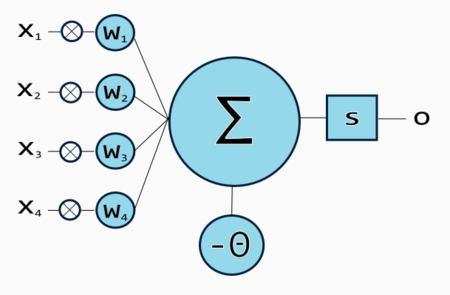
\includegraphics[width=10cm]{images/neuron.png}
\caption[A single neuron]{A single neuron showing weighted inputs from other neurons on the left. These form a summation of which the bias threshold $\theta$ is withdrawn. Finally the activation function \emph{s} decides if to set the binary output active.}
\label{fig:neural-Neuron}
\end{figure}
The central part of an artificial neural network (ANN) is the neuron, as pictured in figure~\ref{fig:neural-Neuron}.
A neuron can be considered as a single computation unit.
It begins by summing up all weighted inputs, and thresholding the value for some constant threshold $\theta$.
Then a transfer function is applied which sets the binary output if the input value is over some limit.

In the case of Boltzmann machines the activation function is stochastic and the probablility of a neuron being active is defined as follows:
\[
p_{i=on} = \frac{1}{1+e^{-\frac{\Delta E_{i}}{T}}}
\]
$E_i$ is the summed up energy of the whole network into neuron $i$, which is a fully connected to all other neurons.
A neural network is simply a collection of nodes interconnected in some way.
All weights are stored in a weight matrix, describing connections between all the neurons.
T is a temperature constant controlling the rate of change during several evaluations with the probability $p_{i=on}$ during simulation.
$E_i$ is defined as follows \cite{boltzmann2}:
\[
\Delta E_{i} = \sum_{j} w_{ij} s_{j} - \theta
\]
where $s_j$ is a binary value set if neuron $j$ is in a active state, which occurs with probability $p_{i=on}$, and $w_{ij}$ are weights between the current node and node $j$. $\theta$ is a constant offset used to control the overall activation.

The state of every node and the associated weights describes the entire network and encondes the problem to be solved.
In the case of Sudoku there is a need to represent all 81 grid values, each having 9 possible values.
The resulting $81*9=729$ nodes are fully connected and have a binary state which is updated at every discrete timestep.
Some of these nodes will have predetermined outputs since the initial puzzle will fix certain grid values and simplify the problem.
In order to produce valid solutions it is necessary to insert weights describing known relations.
This is done by inserting negative weights, making the interconnected nodes less likely to fire at the same time, resulting in reduced probability of conflicts.
Negative weights are placed in rows, columns, 9x9 subgrids, and between nodes in the same square, since a single square should only contain a single active digit.\\

In order to produce a solution the network is simulated in discrete timesteps.
For every step, all probabilites are evaluated and states are assigned active with the given probability.
Finally the grid is checked for conflicts and no conflicts implies a valid solution, which is gathered by inspecting which nodes are in a active state.

Even though the procedure detailed above eventually will find a solution, there are enhanced techniques used in order to converge faster to a valid solution.
The temperature, $T$, can be controlled over time and is used to adjust the rate of change in the network while still allowing larger state changes to occur.
A typical scheme being used is simulated annealing \cite{simulatedAnnealing}.
By starting off with a high temperature (typically $T_0 = 100$) and gradually decreasing the value as time progresses, it is possible to reach a global minima.
Due to practical constraints it is not possible to guarantee a solution but simulated annealing provides a good foundation which was used.\\

The temperature descent is described by the following function, where $i$ is the current iteration:
\[
T(i) = T_0 * exp(K_t * i)
\]
$K_t$ controls the steepnes of the temperature descent and can be adjusted in order to make sure that low temperatures are not reached too early.
The result section describes two different decline rates and their respective properties.

There are some implications of using a one-pass temperature descent which was chosen to fit puzzles as best as possible.
Typically solutions are much less likely to appear in a Boltzmann machine before the temperature has been lowered enough to a critical level.
This is due to the scaling of probabilites in the activation function.
At a big temperature all probabilites are more or less equal, even though the energy is vastly different.
With a low temperature the temperature difference will be scaled and produce a wider range of values, resulting in increasing probability of ending up with less conflicts.
This motivates the choice of an exponential decline in temperature over time; allowing solutions at lower temperatures to appear earlier.

\chapter{Method}
Since this report have several aims, this section have been divided into different parts to clearly depict what aspects have been considered regarding the different aims. 
Those sections will also describe in detail how the results was generated. 
Section~\ref{sec:testSetupMethod} is devoted to explaining the test setup which includes hardware specifications but also an overview picture of the setup. 
Section~\ref{sec:comparisonMethod} focuses on how and what aspects of the algorithms where analysed.
Section~\ref{sec:benchmarkPuzzles} explains the process of choosing test data.
The last section (\ref{sec:statisticalAnalysis}) gives an overview of the statistical analyses which was performed on the test data.
This also includes what computational limitations was present and how this effected the results. 

\FloatBarrier
\section{Test setup}
\label{sec:testSetupMethod}
The central part of the test setup is the test framework which extracts timing and tests every algorithm on different puzzles. 
In order to provide flexibility, the test framework was implemented as a separate part, which made it possible to guarantee correct timing and also solving correctness of the algorithms.
All execution times were measured and logged for further analysis.
Since there might be variations in processor performance and an element of randomness in stochastic algorithms, multiple tests were performed on each puzzle. 
Lastly when all values satisfied the given confidence intervals a single value (the mean value) was recorded, gradually building up the solving time distribution.

All tests were run on a system using a Intel Q9550 quad core processor @ 2.83 GHz, 4 GB of RAM running on Ubuntu 10.04 x64.
Both the test framework and all solvers were compiled using GNU GCC with optimizations enabled on the \emph{-O2} level.

\FloatBarrier
\section{Comparison Methods}
\label{sec:comparisonMethod}
Multiple aspects of the results was considered when analysing and comparing the algorithms. The following three sections describes those aspects in more detail. 

\FloatBarrier
\subsection{Solving}
The solving ability of the algorithm is the main interest of this thesis.
This is measured by measuring the time it takes for each Sudoku solver algorithm to solve different puzzles.
By doing that on a represantative set of puzzles one can determine which algorithms are more effective.
Solving ability is often given in the form of a mean value, but since puzzles vary greatly in difficulty this misses the bigger picture.
An algorithm might for instance be equally good at all puzzles and one algorithm might be really good for one special kind of puzzles while performing poorly at others.
They can still have the same mean value which illustrates why that is not a good enough representation of the algorithms effectiveness.
The representation of the algorithms performances are therefore presented in the form of histograms, which shows the frequency at which puzzles fall into a set of time intervalls.
This does not only depict a more interesting view of the Sudoku solvers performance, but also shows possible underlying features such as if the Sudoku solver solves the puzzle with an already known distribution.
This topic are mostly studied for each algorithm, but will also to some extent be compared between the algorithms.

\FloatBarrier
\subsection{Puzzle difficulty}
\label{sec:puzzleDifficulty}
One can often find difficulty ratings associated to Sudoku puzzles in puzzle books etc. 
Those are often based on the level of human solving techniques that are needed to solve the puzzle in question.\cite{difficulty} 
This study will similarly measure the puzzles difficulty, but will not rely on which level of human solving techniques that are needed, but instead on how well each algorithm performs at solving each puzzle. 
The test will primarly consist of determining if certain puzzles are inherently difficult, meaning that all algorithms rate them as hard.
During the implementation process it was discovered that the Boltzmann machine performed much worse than the other algorithms and could therefore not be tested on the same set of puzzles.
The comparison of this aspect is therefore focused on the rule-based and backtrack algorithms.

\FloatBarrier
\subsection{Generation and parallelization}
This is a more theoretical aspect of the comparison and no tests will be done.
It is however still possible to discuss how well the algorithms are suited for generating puzzle and how well they can be parallelized. 
Generation of puzzles is obviously interesting as that is what one has to do to get new Sudoku puzzles.
One can generate Sudoku puzzles in multiple ways, but since this thesis is about Sudoku solving algorithms only generating methods involving such algorithms will be considered.
The primarly way of generating Sudoku puzzles is then by inserting random numbers into an empty Sudoku grid and then attempting to solve the puzzle.

Parallelization is however not entirely obvious why it is of interest. 
Normal Sudoku puzzles can be solved in a matter of milliseconds by the best Sudoku solvers and one might therefore struggle to see the need for parallelization those solvers. 
This topic is indeed quite unrelevant for normal Sudoku puzzles, but the discussion that will be held about the algorithms might still hold some value.
One might for instance attempt to construct a Sudoku solver for NxN puzzles and as those can quickly get very complex as N increases, one are likely to be in need of computational improvements.  
Since the algorithms to some extent also can be applied to other NP-complete problems, the discussion could also be relevant in determining which type of algorithms are useful for similar problems. 

\FloatBarrier
\section{Benchmark puzzles}
\label{sec:benchmarkPuzzles}
The test data consisted of multiple puzzles that was chosen beforehand.
Since the set of test puzzles can affect the outcome of this thesis it is appropriate to motivate the choice of puzzles.
As was discovered during the study the Boltzmann machine algorithm did not perform as well as the other algorithms and some modifications to which puzzles was used was therefore done.
The backtrack and rule-based algorithms was however both tested on a set of 49151 17-clue puzzles. 
Those was found on \cite{database} and is claimed by the author Royle to be a collection of all 17-clue puzzles that he has been able to find on the Internet. 
The reason for chosing this specific database is because the generation of the puzzles does not involve a specific algorithm but is rather a collection of puzzles found by different puzzle generating algorithms.  
The puzzles are therefore assumed to be represantative of all 17-clue puzzles. 
This assumption is the main motivating factor for chosing this set of puzzles, but there is also other factors that makes this set of puzzles suitable. 
As recently discovered by Tugemann and Civario, no 16-clue puzzle exists which means that puzzles must contain 17 clues to have unique solutions.\cite{17clueProof}  
\label{sec:puzzleDifficulty}
As discussed under section~\ref{sec:puzzleDifficulty}, difficulty rating is poorly measured by the number of clues in a puzzle, but one can however see a correlation between the number of clues and the difficulty.\cite{difficulty}
This means that the chosen set of 17-clue puzzles shall contain some of the hardest Sudoku puzzles that exists.
This is ofcourse a wanted feature since the algorithms are then tested on puzzles of all difficulty levels.

As mentioned, the Boltzmann machine could not solve 17-clue puzzles effieciently enough which forced a change in test puzzles. The Boltzmann machine algorithm was therefore tested on 400 46-clue puzzles. Those where generated from a random set of the 17-clue puzzles used for the other algorithms and is therefore assumed that they are not biased towards giving a certain result.
One problematic aspect is that they can probably not be said to represent all 46-clue puzzles.
This is because they are generated from puzzles that are already solvable and the new puzzles should therefore have more logical constraints then the general 46-clue puzzle.
Most 46-clue puzzles already have a lot of logical constraints due to the high number of clues and the difference of the generated puzzle and the general 46-clue puzzle is therefore thought to be negligible.
\FloatBarrier
\section{Statistical analysis}
\label{sec:statisticalAnalysis}
Due to several reasons statistical analyses is required to make a rigouros statement about the results. 
This is mainly due to two reason.
Firstly the results contain a very large dataset and secondly there are some randomness in the test results which can only be dealt with by using statistical models. 
Most statistical tests give a confidence in the results to depict how surely one can be about the results of the statistical test. Naturally a higher confidence and more precise results leads to higher requirements on the statistical test. As described in section 3.4.2 some of the statistical tests have been limited by computational constraints and a lower confidence level in combination with a more inprecise result have therefore been needed for those tests.

\FloatBarrier
\subsection{Statistical tests}
\label{sec:statisticalTests}
This section explains which statistical tests and methods are used in the study.
The first statistical method that is applied is to make sure that variance in processor performance does not affect the results considerable. 
This is done by measuring a specific algorithms solving time for a specific puzzle multiple times. 
The mean value of those times are then calculated and bootstraping are used to attain a 95\% confidence interval of 0.05 seconds. 
The reason bootstraping is used is because it does not require the stochastic variable to be a certain distribution. 
This is necessary since the distribution of the processor perfomance is unknown and also since the distribution might vary between different puzzles. The solving time may also vary greatly if the algorithm uses a stochastic approach, such as the Boltzmann machine algorithm.

The meanvalues are then saved as described in section~\ref{sec:testSetupMethod}.
It is now that the real analyses of the algorithms begins. 
Even if the representation of the results does not really classify as a statistical method it is appropriate to mention that the results are displayed as histograms which means that the data are sorted and devided into bars of equal width. 
For this study this means each bar represents a fixed size solution time intervall. 
The height of the bars are proportional to the frequency data points falls into that bar's time intervall.
After the histogram are displayed one can easily compare the results between different algorithms and also consider the distribution of the solution times of individual algorithms.\\
The first thing one might think of looking for is how the different algorithms compare in solving ability. 
This means that one want to find out if one algorithm is better than other algorithms. 
Since the distribution is unknown one has to rely on more general statistical tests. 
One of those are Wilcoxons sign test. 
This makes use of the fact that the difference in solving times between two algorithms will have a mean value of 0 if there is no difference between the two algorithms. 
The tests uses the binomial distribution to see if the sign of the difference is unevenly distributed.
The null hypothesis is that the two algorithms perform equally and to attain a confidence for the result one compute the probability that one falsely rejects the null hypothesis given the test results.
\\
Difficulty distribution among the puzzles can be seen by looking at the histograms for each algorithm.
One aspect that is of interest is if some of the puzzles are inherently difficult, or easy, independent on which algorithm is used for solving it.
The method used for determining this is built on the fact that independent events, say A and B, must follow the following property:
\[
P(A \cap B) = P(A) P(B)
\] 
To illustrate what this means for this thesis, lets consider the following scenario.
A is chosen to be the event that a puzzle is within algorithm one's worst 10\% puzzles.
B is similiarly chosen to be the event that a puzzle is within the 10 \% worst puzzles for algorithm 2.
The event $A \cap B$ shall if the algorithms are independent then have a probability of 1\%.
To test if this is the case one again uses the binomial distribution with the null hypothesis that the two algorithms are independent.
This hypothesis is then tested in the same way as the above described method (wilcoxons sign test).

\FloatBarrier
\subsection{Computational constraints}
The computational constraints of the computations done in relation to this thesis mainly originates from processor performance.
This was as aboved described handled by running multiple tests on the same algorithm with each puzzle.
The problem is that bootstraping which was used to determine confidence levels of the measured mean value, requires a large data set to attain a high confidence level. 
At the same time the puzzle set was very big which required a compromise which lead to a confidence interval of 0.05 seconds to a confidence level of 95\%. The number of tests that was allowed for each puzzle was also limited to 100 tries.
The puzzles that could not pass the requirements for the confidence interval was marked as unstable measurment.
\\
Another problematic aspect concerning computational constraints is the running time for each algorithm.
During the implementation phase it was discovered that the backtrack algorithm was slow for some puzzle with 17 clues and the Boltzmann machine was discovered to be much to slow for all 17 clue puzzle.
The way this was handled was by setting a runningtime limit of 20 seconds for each test run for the backtrack solver.
The Boltzmann machine required a more dramatic solution and the test puzzles was exchanged with ones with 51 clues instead of 17. 
This was quite unfortunate as this leaves some of the comparison aspects with only two algorithms.

\chapter{Analysis}
In this section multiple results are presented together with a discussion about how the results could be interpreted. 
Section~\ref{sec:timeDistributions} is devoted to presenting how different algorithms perform. 
Section~\ref{sec:comparisonAnalysis} show how the algorithms performs relative to the each other and discusses different aspect of comparison.
Section~\ref{sec:difficultyAnalysis} explores the idea of difficulty rating and the concept of some puzzles being inherently difficult.
Section~\ref{sec:generation} compares the algorithms by how well they are suited for generation and parallelizing.

\FloatBarrier
\section{Time distributions}
\label{sec:timeDistributions}
To get an idea of how each algorithm performs one can plot the solving times in a histogram. 
Another way of displaying the performance is to sort the solving times and plot puzzle index versus solving time. 
Both of those are of interest however since they can reveal different things about the algorithms performance. 
 
\FloatBarrier
\subsection{Rule-based solver}
The rule-based solver was by far the fastest algorithm in the study with a mean solving time of 0.02 seconds.
Variation in solving time was also small with a standard deviation of 0.02 seconds. 
It solved all 49151 17-clue puzzles that was in the puzzle database used for testing and none of the puzzles resulted in a unstable measurement of the solving time.
\\
%The time distribution for the rule-based solver can be seen in 
%figure ~\ref{fig:rulebasedHistogram}, ~\ref{fig:rulebasedHistogram2} and ~\ref{fig:rulebasedIndices}.
Figure~\ref{fig:rulebasedHistogram} is a histogram on a logaritmic scale that shows how the rule-based solver performed over all test puzzles.
As one can see there is a quite samll time intervall at which most puzzles are solved.
This is probably due to the use of logic rules with a polynomial time complexity.
When the solver instead starts to use guessing the time complexity is changed to exponential time and it is therefore reasonable to believe that the solving time will then increase substantially.
As will be seen in section~\ref{sec:backtrack} the backtrack algorithm have a similar behaviour which is also taken as a reason to believe that the rule-based solver starts to use guessing after the peak.
Guessing might ofcourse be used sparingly at or even before the peak, but the peak is thought to decrease as a result of a more frequent use of guessing.
\\
\begin{figure}[here] 
\noindent\makebox[\textwidth]{%
\begin{tabularx}{1.25\textwidth}{XX}
    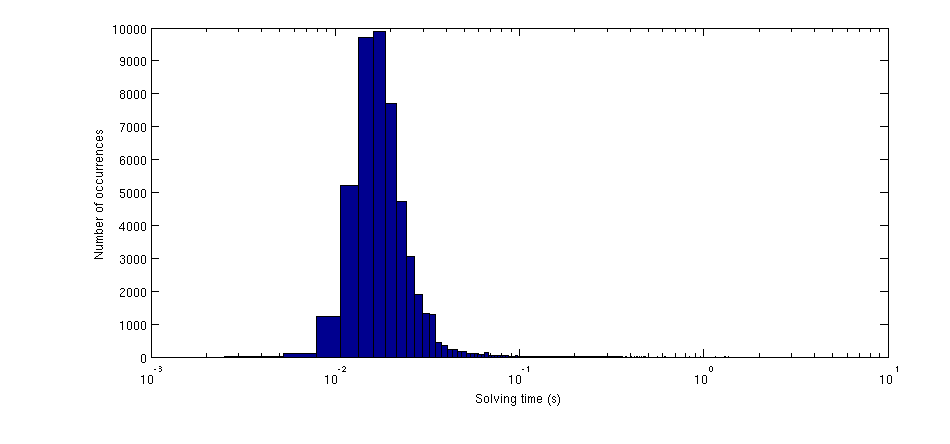
\includegraphics[width=15cm]{images/rulebased_histogram.png}
\end{tabularx}}
\vspace{-25pt}
\caption[Histogram with solving times for rule-based solver]{A histogram displaying the solving times for the rule-based solver. The x-axis showing solving time have a logaritmic scale to clearify the result. The reader shall note that this makes the bars in the histograms' widths different, but they still represent the same time interval. All puzzles was solved and none had an unstable measurment in running time. The confidence level for the measured solving times was 95 \% at an intervall of 0.05 seconds.}
\label{fig:rulebasedHistogram}
\end{figure}

Figure~\ref{fig:rulebasedHistogram2} shows a zoomed in view of figure~\ref{fig:rulebasedHistogram} but with a linear time scale.
The histogram's bars also has half the width compared to figure~\ref{fig:rulebasedHistogram}.
As one can see the histogram begins at the end of the peak that is illustrated in figure~\ref{fig:rulebasedHistogram}.
This is to illustrate that the histogram continues to decrease.
The histogram also illustrates that the maximum time was 1.36 seconds, but that only very few puzzles have a solving time close to that.
As can be seen most puzzles will have solving time less than 0.4 seconds.
\\
\begin{figure}[here] 
\noindent\makebox[\textwidth]{%
\begin{tabularx}{1.25\textwidth}{XX}
    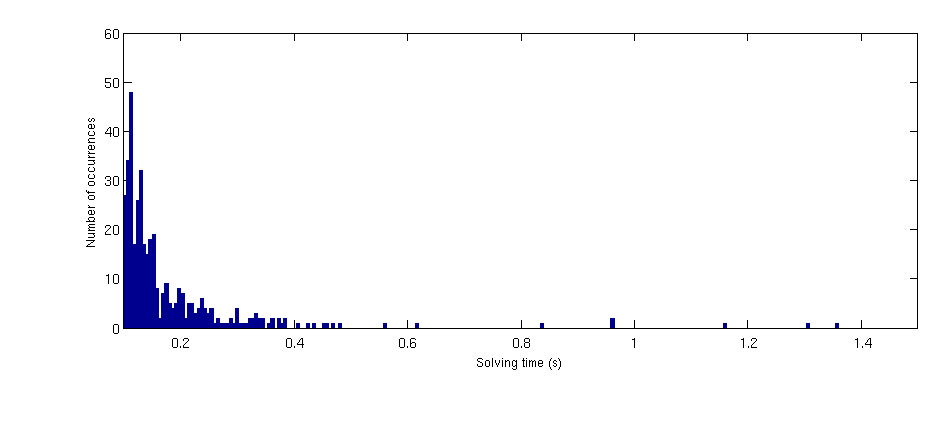
\includegraphics[width=16cm]{images/rulebased_histogram2.png}
\end{tabularx}}
\vspace{-40pt}
\caption[Histogram with solving times for rule-based in a zoomed in view]{A zoomed in view of the histogram in figure ~\ref{fig:rulebasedHistogram} showing the rule-based solvers time distribution among all 49151 puzzles. The bars represent half the time intervall compared to figure ~\ref{fig:rulebasedHistogram}. All puzzles was solved and none had an unstable measurment in running time. The confidence level for the measured solving times was 95 \% at an intervall of 0.05 seconds.}
\label{fig:rulebasedHistogram2}
\end{figure}

\FloatBarrier
Another way to visualize the result is shown in figure~\ref{fig:rulebasedIndices}.
The figure have plotted the puzzle indices sorted after solving time against their solving times.
Note that the y-axis is a logaritmic scale of the solving time.
As in figure~\ref{fig:rulebasedHistogram2} one can see that only a few puzzles had relatively high solving times.
This picture also more clearly illustrates the idea explored above.
Namely that the algorithm will increase its solving times fast at a certain point.
That point is as mentioned thought to be the point where the solver starts to rely more upon guessing then the logical rules.
From that statement one can conclude that only a small portion of all sudoku puzzles are difficult in the sense that the logic rules that the rule-based solver uses is not enough.
\\
\begin{figure}[here] 
\noindent\makebox[\textwidth]{%
\begin{tabularx}{1.1\textwidth}{XX}
    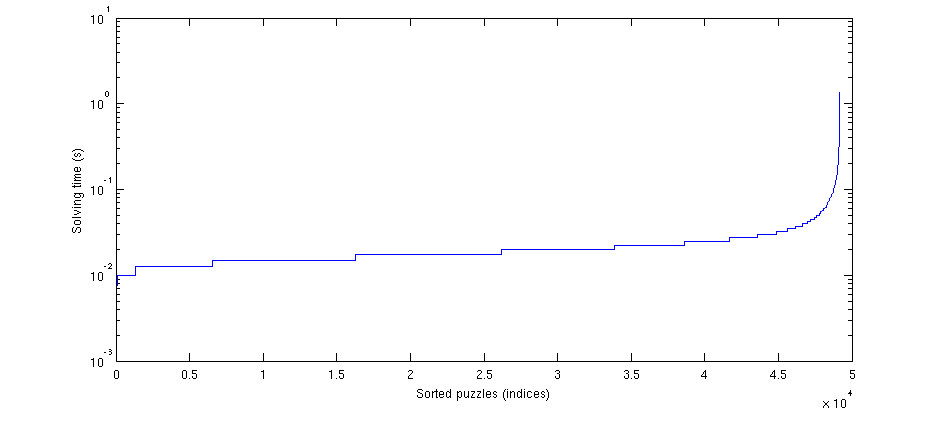
\includegraphics[width=15cm]{images/rulebased_sortedindices.png}
\end{tabularx}}
\vspace{-25pt}
\caption[Plot of solved puzzles using rule-based solver]{The x-axis is the indices of the puzzles when sorted according to the solving time for the rule-based solver. The y-axis shows a logaritmic scale of the solving time for each puzzle. All 49151 puzzles was solved and none had an unstable measurment in running time. The confidence level for the measured solving times was 95\% at an intervall of 0.05 seconds.}
\label{fig:rulebasedIndices}
\end{figure}

\FloatBarrier
\subsection{Backtrack solver}
\label{sec:backtrack}
The backtrack algorithm was the second most effiecent algorithm of the tested algorithms.
It had a mean solving time of 1.66 seconds and a standard deviation of 3.04 seconds.
The backtrack algorithm was tested on the same set of puzzles as the rule-based algorithm, but did not manage to solve all puzzles within the time limit that was set to 20 seconds.
It had $142$ puzzles with unstable measurments and was unable to solve $1150$ puzzles out of all $49151$ puzzles.
In figure~\ref{fig:backtrackDistribution} the solving time is plotted against the number of occurrences within each time intervall.
Each data point represents 0.5 seconds and one shall also note that the y-axis is a logaritmic scale of the time.
With that said one can see that the solving times seems to be decreasing at a approximately exponential rate.
That is linear in the diagram as the y-axis is a logaritmic scale.

\begin{figure}[here] 
\noindent\makebox[\textwidth]{%
\begin{tabularx}{1.20\textwidth}{XX}
    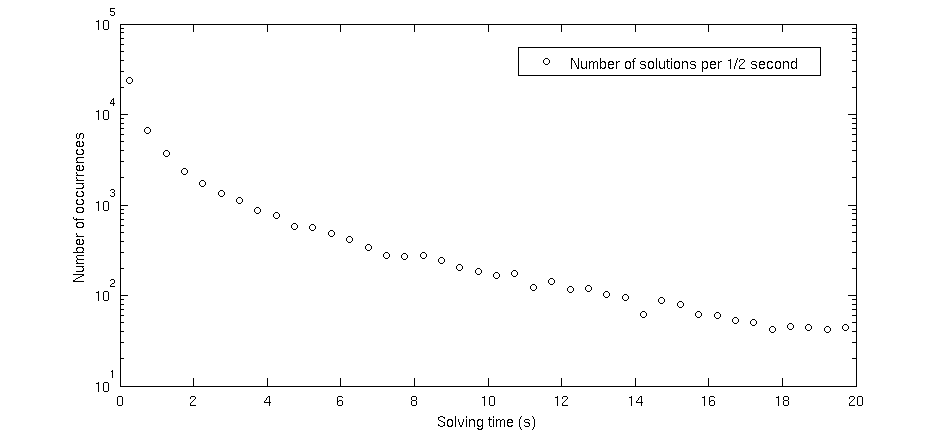
\includegraphics[width=16cm]{images/backtrack_distribution.png}
\end{tabularx}}
\vspace{-15pt}
\caption[Plot of backtrack results]{A plot similar to a histogram showing the results of the backtrack solver for all solved puzzles. The algorithm left $1150$ unsolved (time limit was 20 seconds) and 142 with unstable measured solving times out of all 49151 puzzles. Note that the y-axis is a logaritmic scale of the solving times. The confidence level for the measured solving times was 95\% at an intervall of 0.05 seconds.}
\label{fig:backtrackDistribution}
\end{figure}

\FloatBarrier
One might also plot the indices of the puzzles sorted according to solution time against their solution times, as in figur~\ref{fig:rulebasedIndices} showing the corresponding result for the rule-based solver.
As one can see in figure~\ref{fig:backtrackIndices} the solving times increase in a similar fasion to the rule-based solver.
Note that figure~\ref{fig:rulebasedIndices} uses a logaritmic scale while this figure (figure~\ref{fig:backtrackIndices}) does not.
The solving times are higher thought, and the increase is not as abrupt as for the rule-based algorithm.
One can also see that the solving times reach the time limit of 20 seconds.
This probably means that the solving times would have continued to increase for the last $1150$ unsolved puzzles.
If one uses extrapolation, the time it would take to solve the last puzzle would be very large since the slope is very large at the last solved puzzles. 
As this is a deterministic algorithm one knows that their is a limit to how long a puzzle may take to solve, but as that limit is not known it is impossible to know what the solving times of the last puzzle would be.
There is however no reason to believe that this limit is close to 20 seconds so the solving times of the last puzzles may very well be multiple hours or worse.
\\
\begin{figure}[here] 
\noindent\makebox[\textwidth]{%
\begin{tabularx}{1.20\textwidth}{XX}
    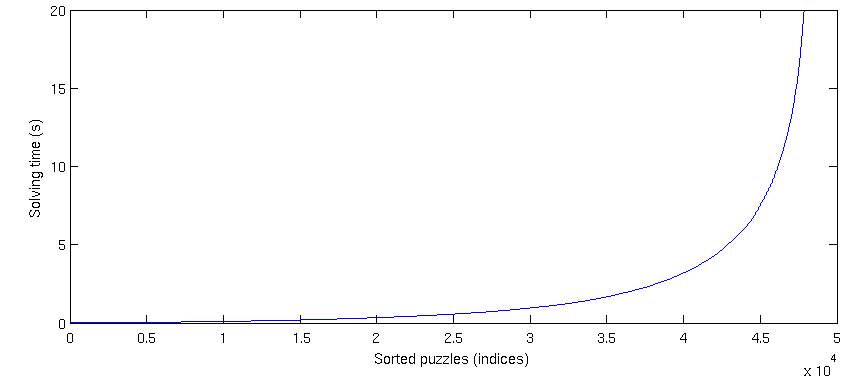
\includegraphics[width=16cm]{images/backtrack_sortedindices.png}
\end{tabularx}}
\vspace{-15pt}
\caption[Plot of backtrack solving times]{The backtrack algorithm's puzzles plotted against their solving times. The x-axis is the indices of the puzzles when sorted according to solving times. Note that this plot is different from figure~\ref{fig:rulebasedIndices} as this plot have a linear y-axis. The plot shows the distribution of the solved puzzles with stable measurements of their running times. There where $49151$ puzzles in total tested and $1150$ of those were unsolved (time limit was 20 seconds) and $142$ of those had unstable measurments of their solving times. The confidence level for the measured solving times was 95\% at an intervall of 0.05 seconds.}
\label{fig:backtrackIndices}
\end{figure}

\FloatBarrier
From figure~\ref{fig:backtrackDistribution} and figure~\ref{fig:backtrackIndices} one may think that the solution times are exponentially distributed since both of those figures hinted that the probability of finding puzzles with higher solving times decreased exponentially.
As figure~\ref{fig:backtrackExponential} shows this is not the case.
The figure instead shows that the distribution for the backtrack algorithm's solving times seems to have a higher concavity than the fitted exponential distribution have.

\begin{figure}[here] 
\noindent\makebox[\textwidth]{%
\begin{tabularx}{1\textwidth}{XX}
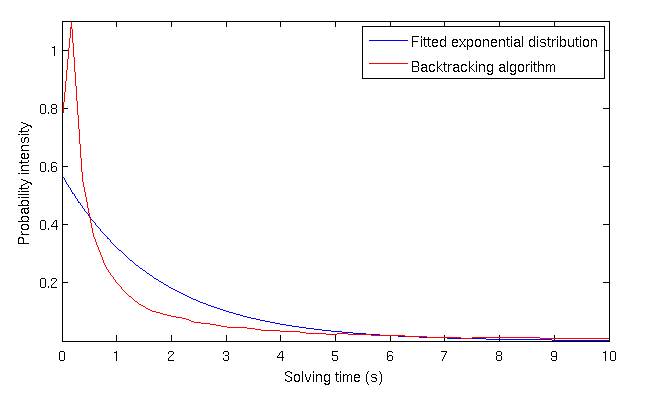
\includegraphics[width=13cm]{images/backtrack_exponential.png}
\end{tabularx}}
\vspace{-15pt}
\caption[Backtrack solving times as a probability intensity function]{The distribution of the backtrack algorithm's solving times as a probability intensity function plotted together with a fitted exponential distribution. 
The fitted exponential distribution was obtained by using the reciprocal of the mean value of the solving times for the backtrack algorithm as $\lambda$ (which is the parameter used in the exponential distribution). 
The $1150$ unsolved puzzles and the $142$ puzzles with unstable measurement out of the $49151$ puzzles was left out of this computation. 
The confidence level for the measured solving times was 95 \% at an intervall of 0.05 seconds.}
\label{fig:backtrackExponential}
\end{figure}

\FloatBarrier
\subsection{Boltzmann machine solver}
The Boltzmann machine solver did not perform as well as the other algorithms and therefore required to be tested on puzzles with 46 clues, in order to have reasonable execution times.
Two different parameter settings were tested and the results demonstrates some important differences in solving capabilities.
All results share the time limit of 20 seconds, with worse results or unstable measurements not shown.

\begin{figure}[here] 
\noindent\makebox[\textwidth]{%
\begin{tabularx}{1.20\textwidth}{XX}
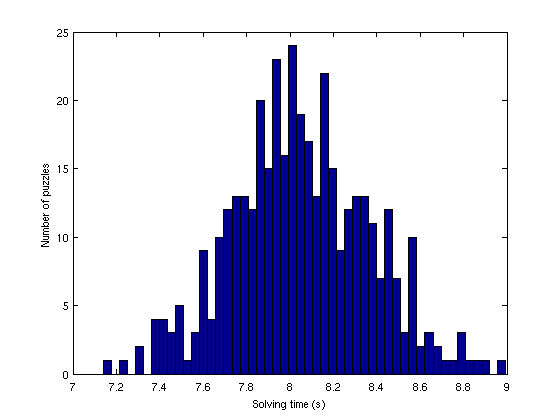
\includegraphics[width=12cm]{images/boltzmann_fast.png}
\end{tabularx}}
\vspace{-15pt}
\caption[Histogram with distribution of Boltzmann machine with fast decline]{Histogram showing distribution of Boltzmann machine results running on 400 puzzles with 46 clues using a fast decline in temperature. All results belong to a 95\% confidence interval of 1 second. The image only contains puzzles being solved under the 20 second limit, which were 98.5\% of all tested puzzles.}
\label{fig:boltzmannFast}
\end{figure}

Figure \ref{fig:boltzmannFast} shows all resulting execution times, belonging to a 95\% confidence interval of 1 second, when using a fast decline in temperature.
The solved puzzles represent 98.5\% of all tested puzzles, with no measurements being unstable.
These values were produced using a temperature decline constant of $K_t = -0.000035$.

\begin{figure}[here] 
\noindent\makebox[\textwidth]{%
\begin{tabularx}{1.20\textwidth}{XX}
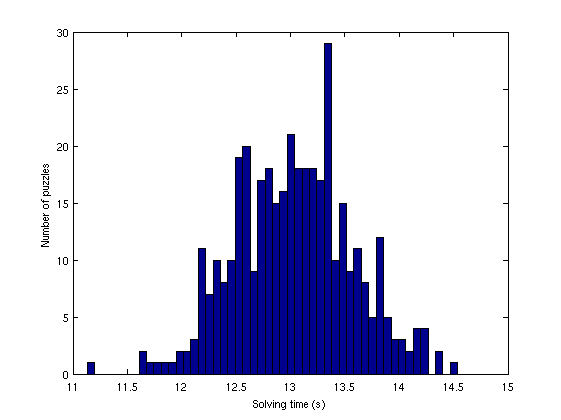
\includegraphics[width=12cm]{images/boltzmann_medium.png}
\end{tabularx}}
\vspace{-15pt}
\caption[Histogram with distribution of Boltzmann machine with slow decline]{Histogram showing distribution of Boltzmann machine results running on 400 puzzles with 46 clues using a slow decline in temperature. All results belong to a 95\% confidence interval of 1 second. The image only contains puzzles being solved under the 20 second limit, which were 97.5\% of all tested puzzles. Another 2\% were unstable measurements.}
\label{fig:boltzmannMedium}
\end{figure}

Figure \ref{fig:boltzmannMedium} show the corresponding histogram for a temperature constant of $K_t = -0.000025$.
The resulting distribution if slightly shifted to higher solving times, indicating that less puzzles are solved at a lower temperature.
A total of 97.5\% of all puzzles were solved.
This slower temperature decline resulted in 2\% unstable measurements, which is an increase over the faster version. \\

Given the requirement of a less strict confidence interval, due to higher variance within estimates of single puzzles, there is a higher margin of error in the results.
Inspection of the two different distributions indicates that all solved puzzles are completed within their respective small intervals, with further conclusions being limited by the margin of error. \\

A strong reason for the big representation of solutions clustered at a low temperature is the general layout of a Boltzmann solver.
Given that solutions are more likely to be observed at lower temperatures, as explained in the background section, it is expected to have more solutions at the end of the spectrum.
For example by studying the fast solver it is observable that the medium value of 8 seconds is equivalent to a temperature of about 0.5\%.
This leads to a conclusion of this being a critical temperature for solutions to stabilze.
After the intervals of critical temperatures there were no puzzles being solved within the limit of 20 seconds.

\FloatBarrier
\section{Comparison}
\label{sec:comparisonAnalysis}
As the reader have already seen in section~\ref{sec:timeDistributions} the algorithms performances relative to each other seems quite clear.
The rule-based algorithm performed best, the backtrack algorithm was next and the Boltzmann machine performed worst.
It is however still interesting to see plots of the differences between the algorithms.
Figure~\ref{fig:comparison} is one such plot which in this case shows the difference between the backtrack algorithm and the rule-based algorithm. The differences in solving time are sorted and plotted with the sorted differences indices as the x-axis. Note also that the y-axis is a logaritmic scale of the solving time differences.
This also means that zero and negative numbers is not included which in turn means that one cannot see the puzzles where the backtracking algorithm performed better than the rule-based algorithm.
The backtrack did however perform better than the rule-based algorithm at $2324$ puzzles.
This is interesting as that means that the rule-based algorithm is wasting time checking logic rules which will not be of any use.
The reason why this can be concluded is because the rule-based and backtracking algorithm is in fact implemented as the same algorithm with the only difference that the rule-based algorithm uses two additional rules in addition to guessing.
Since the guessing is equally implemented for both the only way the rule-based algorithm can be slower is by checking rules in situations where they cannot be applied.
\\

\begin{figure}[here] 
\noindent\makebox[\textwidth]{%
\begin{tabularx}{1.20\textwidth}{XX}
    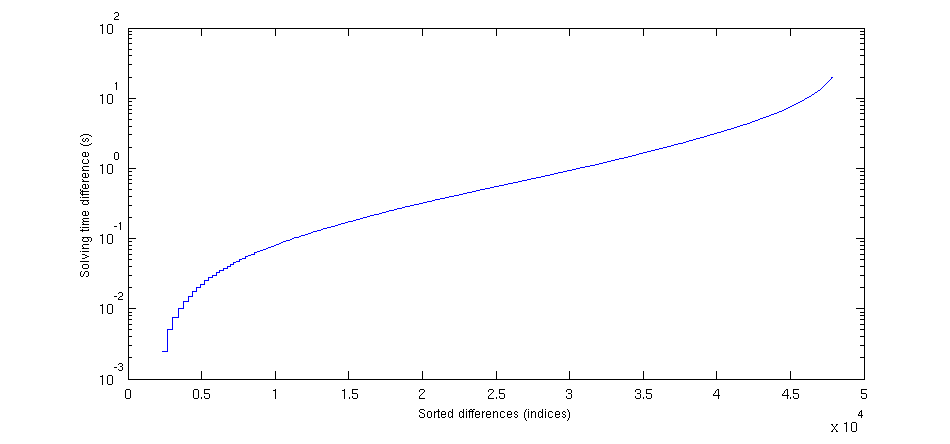
\includegraphics[width=15cm]{images/comparison.png}
\end{tabularx}}
\vspace{-15pt}
\caption[Plot of puzzle difference between solvers]{Plot of the difference for each puzzle that was solved by both the backtrack algorithm and the rule-based algorithm. Since the rule-based algorithm solved all puzzles with no unstable measurement, it was the backtrack algorithm that limited the puzzles used in this plot. The backtracking algorithm did not solve $1150$ puzzles and had $142$ unstable measurements of its solving time. Both algorithm was tested on a total of $49151$ puzzles with a measurement of their solving time with a confidence intervall of 0.05 seconds to the confidence level of 95\%.
The difference is the backtrack algorithm's solving time minus the rule-based algorithm's solving time. Note also that negative numbers are not included since it is a logaritmic scale.}
\label{fig:comparison}
\end{figure}

Even if figure~\ref{fig:comparison} is quite clear on the matter one might want to do a statistical test for determining that the rule-based algorithm is indeed better than the backtrack algorithm.
If one does this with the proposed method in section~\ref{sec:statisticalTests}, namely Wilcoxons sign test, one obtain a confidence level much higher than 99.9\% meaning that one with certainty can say that the rule-based algorithm is better than the backtrack algorithm as expected.
Another interesting aspect of figure~\ref{fig:comparison} is that some puzzles that are very difficult for the backtracking algorithm are easy for the rule-based algorithm.
This means that the rule-based algorithm makes use of the naked tuple rule.
This can be deduced from the fact that the naked single rule is implicitly applied by the backtracking algorithm because of the way it chooses which square to guess at (it chooses the square with least candidates and in the case of a naked single there is only one candidate).

\FloatBarrier
\section{Puzzle difficulty}
\label{sec:difficultyAnalysis}
Both the backtrack solver and the rule-based solver was runned on the same set of puzzles.
One interesting aspect to study is to see if some of those puzzles are difficult for both algorithms or if the algorithms are independent when it comes to which puzzles they perform well at.
Even if the rule-based solver uses backtrack search as a last resort it is not clear whetever the most difficult puzzles correlates between the two algorithms.
The reason for this is because a puzzle can be very hard for the backtrack algorithm, but still trivial for the rule-based solver. 
This has to do with the naked tuple rule in the rule-based solver that quickly can reduce the number of candidates in each square.
\\
To test for independence the statistical method described in section~\ref{sec:statisticalTests} is used.
The measurements shows that about 20\% of the worst 10\% puzzles is common for the two algorithms. 
This hints that some puzzles indeed are inherently difficult regardless of which of the two algorithms are used.
If that would not have been the case only 10\% of the worst puzzles for one algorithm shall have been among the 10\% worst puzzles.
The statistical test also confirms this with a high confidence level of 99.9\%.
\\
While there is interest to correlate results of the Boltzmann machine solver with others, there are difficulties with doing this.
Considering the large variance in running time for individual puzzles there is little room for statistical significance in the results.

\section{Generation and parallelization}
\label{sec:generation}
As already mentioned no tests was performed to measure the algorithms puzzlegenerating abilities or their improvement when parallelized.
Those are however qualities that can be discussed purely theoretically.
\subsection{Generation}
When generating puzzle one has to make sure that the generated puzzle is valid and has a unique solution.
Puzzles with multiple solutions are often disregarded as Sudoku puzzles and are also unpractical for human solvers since one must guess during the solving process to be able to complete the puzzle. The generation process can be implemented multiple ways, but since this thesis is about Sudoku solving algorithms only this viewpoint is presented.
The way one generates a puzzle is by randomly inserting numbers into an empty Sudoku board and then trying to solve the puzzle. If successful the puzzle is valid and one would then want to find out if the solution is unique. 
Both the rule-based solver and backtrack solver can do this by backtracking even thought a solution was found. This practically means that they can search the whole search three to guarantee that all possible solutions were considered.
The rule-based solver does this much faster since it can apply logical rules to rule out some part of the search three.
Stochastic algorithms such as the Boltzmann machine solver can not do this as easily and are therefore not considered suitable for generation.
If one attempted to use the Boltzmann machine for checking validity and backtracking for checking uniqueness, the result would be that the backtracking would have to exhaust all possible solutions anyway and no improvement would have been made.
Another problem with generation with the Boltzmann machine solver is that it can not know if it is ever going to find a solution.
The solver might therefore end up in a situation where it can not proceed, but where a solution for the puzzle still exists.
If the solver was allowed to continue it will eventually find the solution, but as the solver will have to have a limit to function practically it is not suitable for generation.
As described the Boltzmann machine uses puzzles generated from already existing puzzles.
Empty squares in a valid puzzle is filled in by the correct numbers by looking at the solution of the puzzle that have been obtained previously with any algorithm.
This is a kind of generation even if it is not generally considered as generation.
It is however applicable for generating easier puzzles from a difficult puzzle.

\subsection{Parallelizing}
Parallelization of algorithms is interesting mainly because one might want to use similar algorithms in other problems.
There is mainly two ways one can use parallelizing when it comes to Sudoku solving algorithms.
The first and most obvious one is to solve multiple puzzles in parallel.
That is however not parallelizing of the algorithms themselves and will therefore not be discussed.
The other form of parallelizing is separating the algorithms into parts, which are then run in parallel and the result are then combined.
This might be easy to do for some algorithms, but the separation into parts that whose results could then be combined is not necessarily something that can be done for all algorithms.
All the algorithms in this study does however have some possibilities when it comes to parallelizing them.
The rule-based algorithm could for instance check multiple rules for multiple regions at once.
This is unproblematic since the result can easily be combined by applying the results of all rules on the original puzzle.
Since it may be separated into one thread for each rule for each region (if more advanced rules are used they may require the whole puzzle instead of just one region) one will likely have more then enough separation to perform parallelizing at required level.
\\
The backtracking algorithm may be parallelized by separating the search three and searching each branch in parallel.
One can then simply combine the results by the knowledge that only one branch can succeed if the puzzle is unique and valid.
Depending on the branching factor in the puzzle it might not always be easy to parallelize the algorithm.
One might however choose a square with the number of candidates wanted to get enough parts for parallelizing.
\\
The Boltzmann machine can also be run in parallel to some extent.
On a high level the solving process goes through all nodes and updates their respective states.
This is done sequentially since the network is fully connected.
By splitting up updating of individual neurons it is possible to have constant number of actions being performed in parallel.
Typically these operations are additions of conflicting nodes and are calculated by traversing the whole Sudoku grid.
\\
The conclusion that can be drawn from this is that all algorithms in this thesis may effectively be parallelized with more or less effort.
All the algorithms can furthermore be parallelized without adding any considerable overhead, meaning that the solving times could be linearly decreasing over the number of threads, up to some amount.

\chapter{Conclusion}
Three different Sudoku solvers have been studied; backtrack search, rule-based solver and Boltzmann machines.
All solvers were tested using a test framework with statistically significant results being produced.
They have shown to be dissimilar to each other in terms of performance and general behaviour.

Backtrack search and rule-based solvers are deterministic and form execution time distributions that are precise with relatively low variance.
Their excecution time was also shown to have rather low variance when sampling the same puzzle repeatedly, which is believed to result from the highly deteministic behaviour.

The Boltzmann machine solver was not capable of solving harder puzzles with less clues within a reasonable timeframe.
A suitable number of clues was found to be 46 with a 20 second execution time limit, resulting in vastly worse general capabilites than the other solvers.
Due to stochastic behaviour, which is a central part of the Boltzmann solver, there was a relatively large variance when sampling the execution time of a single puzzle.
Another important aspect of the Boltzmann is the method of temperature descent, in this case selected to be simulated annealing with a single descent.
This affected the resulting distribution times in a way that makes the probability of puzzles being solved under a certain critical temperature limit high.
The critical temperature was found to be about 0.5\% of the starting temperature, with no puzzles being solved after this interval.

Additionaly two different methods of temperature descent were studied.
The results demonstrates that a slower descent solves more puzzles, even though the execution times are clustered closer to the 20 second execution limit.

All results indicate that deterministic solvers based on a set of rules perform well and are capable of solving Sudokus with a low amount of clues.
Boltzmann machines were found to be relatively complex and requires implementation of temperature descent and adjustment of parameters.

With regards to parallelization it is possible to implement to a varying extent in all algorithms.
The most obvious way of solving several different puzzles in parallel has been used in the test framework.
Parallel solving of individual puzzles require extensive analysis of individual algorithms, but both backtrack and rule-based have shown to inhibit parallelizable properties.
Boltzmann machines can be made parallel on a more fine grain level but are somewhat limited due to synchronous updates.

Deterministic algorithms such as backtrack and rule-based have been discussed in the context of puzzle generation, and are considered to perform well.
This follows by their search structure which can guarantee a unique solution, in opposite of the general stochastic behaviour of Boltzmann machines, that only gives very weak guarantees.

Future work includes studying the behaviour of Boltzmann machines in relation to the final distribution of execution times.
The large variance and stochastic behaviour most likely demands a study with access to large amounts of computational power.
It is also interesting to study the influence of different temperature descent methods used in Boltzmann machines, with restarting being a suitable alternative to endlessly decreasing temperatures.
The rule-based algorithm may be studied in more detail by adding additional rules and also varying the order in which the rules are applied.
The backtrack algorithm may similarly be studied in more detail by adding additional variations on it, which primarly includes how it chooses which square to start each search tree with.


\begin{thebibliography}{99}

\bibitem{complexity}
Takayuki Y, Takahiro S. Complexity and Completeness of Finding Another Solution and Its Application to Puzzles. [homepage on the Internet]. No date [cited 2012 Mar 8]. Available from: The University of Tokyo, Web site: http://www-imai.is.s.u-tokyo.ac.jp/~yato/data2/SIGAL87-2.pdf

\bibitem{17clueProof}
Tugemann B, Civario G. There is no 16-Clue Sudoku: Solving the Sudoku Minimum Number of Clues Problem. [homepage on the Internet]. 2012 [cited 2012 Mar 8]. Available from: University College Dublin, Web site: http://www.math.ie/McGuire\_V1.pdf

\bibitem{enumeration}
Felgenhauer B, Jarvis F. Enumerating possible Sudoku grids. [homepage on the Internet]. 2005 [cited 2012 Mar 8]. Available from: University of Sheffield, Web site: http://www.afjarvis.staff.shef.ac.uk/sudoku/sudoku.pdf

\bibitem{techniques}
Astraware Limited. Techniques For Solving Sudoku. [homepage on the Internet]. 2008 [cited 2012 Mar 8]. Available from:, Web site: http://www.sudokuoftheday.com/pages/techniques-overview.php

\bibitem{boltzmann}
Ekeberg. Boltzmann Machines. [homepage on the Internet]. 2012 [cited 2012 Mar 8]. Available from:, Web site: http://www.csc.kth.se/utbildning/kth/kurser/DD2432/ann12/forelasningsanteckningar/07-boltzmann.pdf

\bibitem{stochastic}
Marwala T. Stochastic Optimization Approaches for Solving Sudoku. [homepage on the Internet]. 2008 [cited 2012 Mar 8]. Available from:, Web site: http://arxiv.org/abs/0805.0697

\bibitem{review}
. An Incomplete Review of Sudoku Solver Implementations. [homepage on the Internet]. 2011 [cited 2012 Mar 8]. Available from:, Web site: http://attractivechaos.wordpress.com/2011/06/19/an-incomplete-review-of-sudoku-solver-implementations/

\bibitem{discrepancySearch}
Harvey W, Ginsberg M. Limited discrepancy search. [homepage on the Internet]. No date [cited 2012 Mar 13]. Available from: University of Oregon, Web site: http://citeseerx.ist.psu.edu/viewdoc/download?doi=10.1.1.34.2426\&rep=rep1\&type=pdf

\bibitem{searchBased}
Cazenave Cazenave T. A search based Sudoku solver. [homepage on the Internet]. No date [cited 2012 Mar 13]. Available from: Université Paris, Dept. Informatique Web site: http://citeseerx.ist.psu.edu/viewdoc/download?doi=10.1.1.64.459\&rep=rep1\&type=pdf

\bibitem{culturalSwarms}
Mantere T, Koljonen J. Sudoku Solving with Cultural Swarms. AI and Machine Consciousness [homepage on the Internet]. 2008 [cited 2012 Mar 13]. Available from: University of Vaasa, Department of Electrical Engineering and Automation Web site: http://www.stes.fi/step2008/proceedings/step2008proceedings.pdf\#page=60

\bibitem{generation}
Morrow J. Generating Sudoku Puzzles as an Inverse Problem. [homepage on the Internet]. 2008 [cited 2012 Mar 13]. Available from: University of Washington, Department of Mathematics Web site: http://www.math.washington.edu/~morrow/mcm/team2306.pdf

\bibitem{database}
Royle G. Minimum Sudoku. [homepage on the Internet]. No date [cited 2012 Mar 13]. Available from: The University of Western Australia, Web site: http://www.math.washington.edu/~morrow/mcm/team2306.pdf

\bibitem{boltzmann2}
Ackley D, Hinton G. A Learning Algorithm for Boltzmann Machines. [homepage on the Internet]. 1985 [cited 2012 Mar 13]. Available from: The University of Western Australia, Web site: http://learning.cs.toronto.edu/~hinton/absps/cogscibm.pdf

\bibitem{sudokuConstruct}
Wang HW, Zhai YZ, Yan SY. Research on Construting of Sudoku Puzzles. Advances in Electronic Engineering, Communication and Management [serial on the Internet]. 2012 [cited 2012 Apr 11].;1 Available from: http://www.springerlink.com/index/L14T86X63XQ7402T.pdf

\bibitem{sudokuDifficulty}
Mantere TM, Koljonen JK. Solving and Rating Sudoku Puzzles with Genetic Algorithms. Publications of the Finnish Artificial Intelligence Society [serial on the Internet]. 2006 [cited 2012 Apr 11].(23) Available from: http://citeseerx.ist.psu.edu/viewdoc/download?doi=10.1.1.100.6263\&rep=rep1\&type=pdf\#page=91

\bibitem{simulatedAnnealing}
Kirkpatrick SK, Gelatt CD, Vecchi MP. Optimization by Simulated Annealing. Science 1983; (13):671-680.

\bibitem{difficulty}
%TODO Patrik: fix this reference
%http://www.sudokuwiki.org/Weekly_Sudoku.asp
blargh
\end{thebibliography}

\appendix
\addappheadtotoc
\chapter{RDF}\label{appA}

\chapter{Source code}
\lstset{language=C++}

All source code used in the project is included below.
Requests for archives can be made over email.
All files are released with the GNU GPLv2 license.

\section{Test Framework}
\subsection{TestFramework.cpp}
\lstinputlisting{../src/test/TestFramework.cpp}
\subsection{TestFramework.h}
\lstinputlisting{../src/test/TestFramework.h}

\subsection{SodukuSolver.cpp}
\lstinputlisting{../src/test/SudokuSolver.cpp}
\subsection{SodukuSolver.h}
\lstinputlisting{../src/test/SudokuSolver.h}

\subsection{Randomizer.cpp}
\lstinputlisting{../src/test/Randomizer.cpp}
\subsection{Randomizer.h}
\lstinputlisting{../src/test/Randomizer.h}

\section{Boltzmann machine}
\subsection{Boltzmann.cpp}
\lstinputlisting{../src/neural/Boltzmann.cpp}
\subsection{Boltzmann.h}
\lstinputlisting{../src/neural/Boltzmann.h}

\subsection{Square.cpp}
\lstinputlisting{../src/neural/Square.cpp}
\subsection{Square.h}
\lstinputlisting{../src/neural/Square.h}

\section{Rule-based / Backtrack}
The backtracking algorithm and the rule-based algorithm uses the same implementation with one exception. When using only backtracking the whileloop in the applyRules function in Rulebased.cpp is commented out.
\subsection{Rulebased.cpp}
\lstinputlisting{../src/rulebased/rulebased2/Rulebased.cpp}
\subsection{Rulebased.h}
\lstinputlisting{../src/rulebased/rulebased2/Rulebased.h}
\subsection{Board.cpp}
\lstinputlisting{../src/rulebased/rulebased2/Board.cpp}
\subsection{Board.h}
\lstinputlisting{../src/rulebased/rulebased2/Board.h}

\end{document}
